\chapter{Lluvias atmosf\'ericas extendidas (EAS)}
\label{ch:easAuger}

\section{Generalidades}

A fines de la década del treinta Pierre Auger observó que la coincidencia de disparo entre detectores de CR separados varios kilómetros era mayor a la esperada para eventos independientes. Explicó éste hecho postulando la existencia de partículas muy energéticas que, al interactuar  en la alta atmósfera, pudieran generar nuevas partículas de alta energía capaces, a su vez, de repetir el proceso. De esta manera se inicia una reacción de multiplicación en cadena que lleva hoy el nombre de lluvia atmosférica extendida (EAS por su sigla en inglés). 

Tras de 70 años de investigación, la estructura y evolución de las cascadas atmosféricas se condidera bien comprendida.
Tras la primera interacción, su desarrollo puede describirse como un núcleo de partículas de alta energía (usualmente hadrónes), que avanza a lo largo del eje de la lluvia produciendo electrones, muones y fotones menos energéticos, pero con mayor momento transverso relativo, que difunden en la dirección radial (ver Fig.~\ref{fig:lluvia1}). Así, las cascadas están formadas por tres componentes: hadrónica, muónica y electromagnética (ver Fig.~\ref{fig:showerSchema}.

La estructura detallada es enormemente complicada y depende de gran cantidad de factores: partícula primaria, profundidad de la interacción, etc.

%
\begin{figure}[ht]
\begin{center}
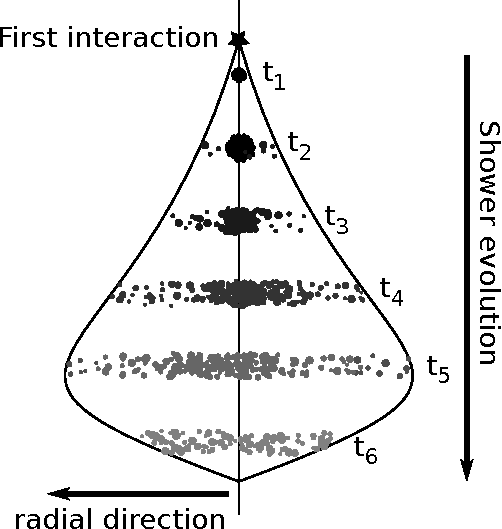
\includegraphics[width=0.75\textwidth]{fig/EASAuger/lluvia1_english.pdf}
\caption{Esquema de la evolución de una cascada atmosférica. Tras la primera interacción se forma un núcleo de partículas de alta energía (usualmente hadrónes), qu avanza a lo largo del eje de la lluvia produciendo nuevas partículas menos energéticas, pero con mayor momento transverso relativo, que difunden en la dirección radial}
\label{fig:lluvia1}
\end{center}
\end{figure}
%
%
\begin{figure}[ht]
\begin{center}
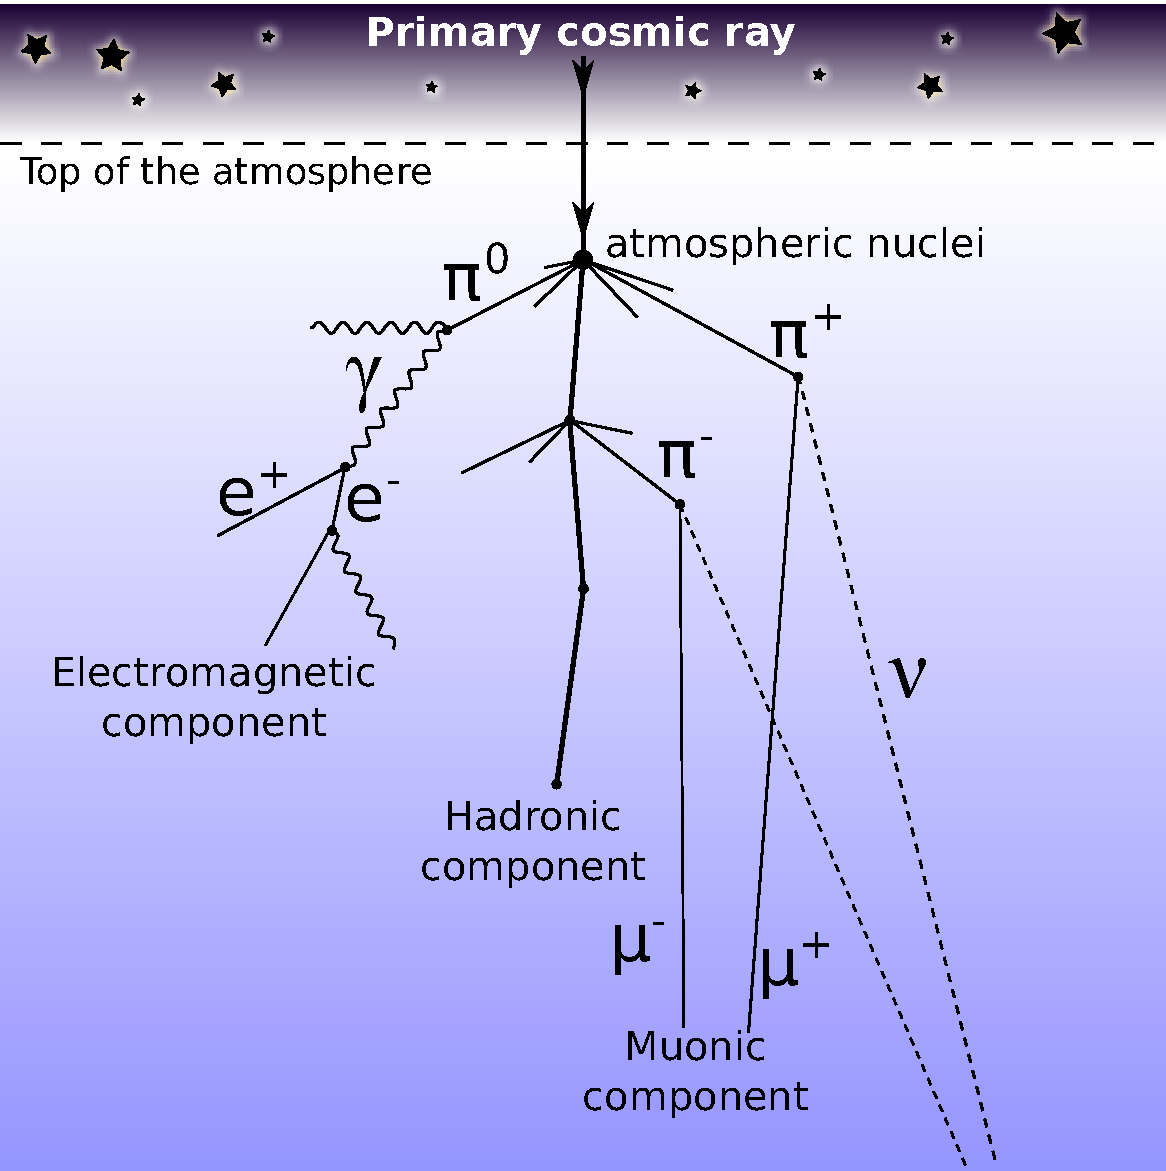
\includegraphics[width=0.75\textwidth]{fig/EASAuger/showerSchema_english.pdf}
\caption{Diagrama esquemático de la estructura de una cascada atmosférica.}
\label{fig:showerSchema}
\end{center}
\end{figure}
%

En la actualidad se considera que la gran mayoría de las cascadas con energía superior a $10^{16}$~eV son iniciadas por UHECR hadrónicos. 
%

En estas lluvias, el número de hadrones aumenta rápidamente durante las primeras etapas de la cascada. Por otro lado, en cada generación, cerca del 30\% de la energía es transferida a la componente electromagnética a través del decaimiento de los $\pi^{0}$ en dos fotones. En las etapas finales, alrededor del 90\% de la energía de la partícula primaria es disipada por la componente electromagnética mediante ionización. La energía restante es transportada por muones y neutrinos originados en el decaimiento de piones cargados que hayan decaído antes de interactuar.

La energía disipada por la componente electromagnética es, con muy buena aproximación, proporcional a la energía de la partícula primaria. Sin embargo, la componente muónica de la lluvia crece más lentamente. Esto se debe a que los muones son principalmete producidos a partir del decaimiento de piones cargados. Debido a la dilatación temporal, los $\pi^{\pm}$ más energéticos tienen menor probabilidad de decaer antes de interactuar y tranferir parte de su energía a la componente electromagnética.


\subsection{Modelo de Heitler}
En esta sección se comentará un modelo simplificado de lluvia desarrollado originalmente por Heitler \cite{hei54} a mediados de los años 50. Si bien el modelo es demasiado simple para obtener resultados cuantitativos precisos, ayuda a comprender cualitativamente la dinámica de las lluvias.

\subsection{Componente electromagnética}
En el cálculo de la evolución de la porción electromagnética de la lluvia se considera que cada electrón radía (bremsstrahlung) un único fotón después de viajar una distancia $d=\lambda \ln(2)$, donde $\lambda\simeq38$~g~cm$^{-2}$ es la longitud de radiación propia del medio\footnote{$d$ es la distancia promedio para la cual un electrón habrá irradiado la mitad de su energía}. Simultáneamente se supone que cada fotón producirá un par $e^{-}$ $e^{+}$ después de recorrer esta misma distancia.
Este proceso se esquematiza en la figura \ref{fig:heilter}.
%
\begin{figure}[ht]
\begin{center}
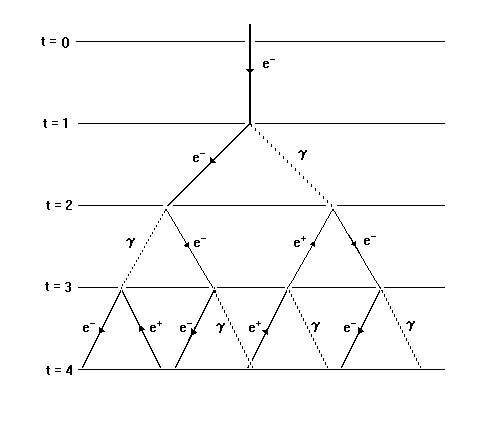
\includegraphics[width=0.75\textwidth]{fig/EASAuger/heilterSchema}
\caption{Esquema del modelo de Heilter. Luego de cada longitud de radiación ($t=nd/\lambda$) los $e^\pm$ emiten un fotón, mientras que los fotones producen un par $e^+e^-$.}
\label{fig:showerSchema}
\end{center}
\end{figure}
%
En ambos casos se toma que la energía se reparte equitativamente entre las partículas hijas. Después de $n$ pasos la lluvia contará con $2^{n}$ partículas entre electrones, positrones y fotones. El modelo considera que la generación de nuevas partículas se detiene cuando la energía perdida por colisiones es mayor que la necesaria para los procesos de bremsstrahlung y producción de pares. En el aire esta energía de corte es de aproximadamente \cant{85}{MeV}. En este punto la cantidad de partículas es máxima y valen las siguientes ecuaciones:
%
\begin{equation}
\label{hi1}
E_p = E_{corte} N_{max} = E_{corte} 2^{n_{max}}
\end{equation}
%
\begin{equation}
\label{hi2}
X_{max}=n_{max} d
\end{equation}
%
con $X_{max}$ la coordenada donde la lluvia alcanza la máxima cantidad de partículas $N_{max}$ luego de $n_{max}$ pasos y $E_p$ la energía del primario.
Despejando $n_{max}$ de (\ref{hi1}) y reemplazando en (\ref{hi2}) se obtiene para Xmax
%
\begin{equation}
\label{hi3}
X_{max} = n_{max} \lambda \ln(2)=\lambda \ln\left(\frac{E_{0}}{E_{corte}}\right)
\end{equation}
%
Las relaciones \ref{hi1} y \ref{hi3}, que pueden resumirse en \ref{hi4}, se recuperan mediante simulaciones a partir de primeros principios.
%
\begin{equation}
\label{hi4}
X_{max} \sim \ln\left(E_{p}\right)
\hspace*{15mm}
N_{max} \sim E_p
\end{equation}
%

\subsection{Componente hadrónica y muónica}
Para modelar la componente hadrónica de la lluvia se utiliza un esquema muy similar al utilizado para la electromagnética.
Se considera que la totalidad de los hadrones son piones ($\pi^{\pm}$ y $\pi^{0}$). Los $\pi^{\pm}$ generan $N \pi^{\pm}$ y $\frac{1}{2}N \pi^{0}$ después de atravesar una feta de atmósfera de ancho $d=\lambda \ln(2)$ siendo $\lambda$ la longitud de interacción para partículas que interactúan fuertemente.
Los $\pi^{0}$ decaen inmediatamente en dos fotones que pasan a formar parte de la componente electromagnética y los $\pi^{\pm}$ continúan la cascada hadrónica hasta que su energía no les permite generar nuevos piones.
En este punto los $\pi^{\pm}$ decaen en muones.
Estos muones, provenientes de $\pi^{\pm}$ de baja energía, forman la totalidad de la componente muónica de la lluvia.
El alto poder de penetración de los muones les permite atravesar la atmósfera sin interactuar en el camino, por lo que generalmente alcanzan la superficie de la tierra antes que la componente electromagnética.

\subsection{Lluvias inclinadas}
\label{sbsc:inclinadas}
%
El término ``lluvias inclinadas'' se refiere a lluvias cuyo ángulo zenital $\theta$ es mayor a $60^{\circ}$.
Con el fin de motivar esta definición es interesante estudiar la cantidad de materia que la lluvia tiene que atravezar hasta alcanzar la tierra como función de $\theta$.
En la figura \ref{fig:slant_depth} se muestra como entre $0^{\circ}$ y $60^{\circ}$ el cambio en la profundidad es un factor $\sim 2$ respecto de su contraparte vertical, \cant{\sim1000}{gcm^{-2}}.
A partir de este punto la profundidad crece rápidamente, alcanzando un factor $\sim 36$ a $\theta=90^{\circ}$.
%
\begin{figure}[h!]
\begin{center}
$
\begin{array}{cc}
 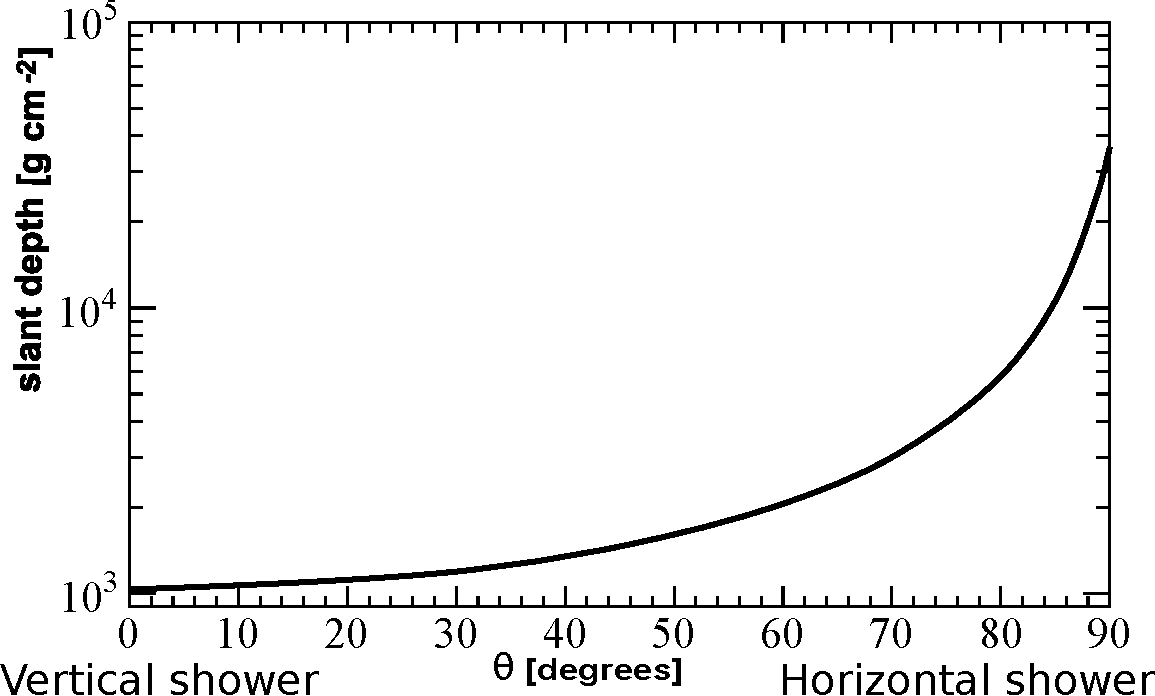
\includegraphics[width=0.47\textwidth]{fig/EASAuger/slant_depth_english.pdf} & 
 \raisebox{0.8\height}{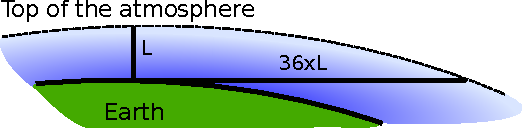
\includegraphics[width=0.47\textwidth]{fig/EASAuger/slantCartoon_english.pdf}}
\end{array}
$
\caption{\textit{Izquierda:} Profundidad atmosférica como función del ángulo zenital $\theta$.
La cantidad de materia crece rápidamente si $\theta>60^{\circ}$.
\textit{Derecha:} Una lluvia completamente horizontal atravieza 36 veces más materia que una vertical.
}
\label{fig:slant_depth}
\end{center}
\end{figure}
%

La mayor parte los rayos cósmicos con energías superiores a \cant{10^{17}}{eV} son protones o nucleos.
Dado que su longitud de interacción en la atmósfera es \cant{\sim50}{gcm^{-2}}, es correcto considerar que estas interactuan en el tope de la atmósfera.
En consecuencia, para lluvias con $\theta>70^\circ$, tanto la componente hadrónica como la electromagnética son completamente absorbidas por la atmósfera, por lo que sólo la componente muónica alcanza el suelo, como se esquematiza en la figura \ref{fig:horizontalHad}.
Como resultado, a nivel del suelo las lluvias horizontales son fundamentalmente diferentes de las verticales.
%
\begin{figure}[h!]
\begin{center}
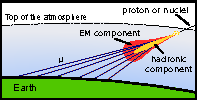
\includegraphics[width=0.7\textwidth]{fig/EASAuger/horizontal2_english.pdf}
\caption{Las lluvias inclinadas producidas por protones o nucleos se inician cerca del tope de la atmósfera.
Las componentes hadrónica y electromagnética se absorben rápidamente, por lo que sólo los muones alcanzan el suelo.
}
\label{fig:horizontalHad}
\end{center}
\end{figure}

\section{Lluvias atmosf\'ericas iniciadas por neutrinos}
\label{sc:easNu}

Existen dos mecanismos principales mediante los cuales los neutrinos pueden iniciar lluvias atmosféricas que puedan producir señales en detectores a nivel del suelo:
\begin{itemize}
 \item Lluvias descendentes: Un neutrino deposita algo de su energía en la atmósfera generando una lluvia descendente cuyas partículas alcanzan el suelo.
 \item Lluvias rasantes: Un neutrino ascendente interactúa con la corteza de la tierra y alguno de sus productos de decaimiento genera una cascada en la atmósfera muy cerca del suelo.
\end{itemize}

\subsection{Lluvias descendentes (DG)}

De acuerdo con el modelo estandar (SM por sus siglas en inglés), los neutrinos interactúan mediante la gravedad y la fuerza débil, pero sólo esta última puede ser utilizada para detectar neutrinos individuales.
Su principal mecanismo de interacción en la atmósfera es la dispersión inelástica profunda (DIS por sus siglas en inglés, \emph{Deep Inelastic Scattering}) con un nucleo de la misma. Los posibles canales se esquematizan en la figura \ref{fig:SM_nu_int} para los diferentes sabores de neutrinos.
En todos los casos, cerca del \cant{20}{\%} de la energía del neutrino primario se transfiere al jet hadrónico mediante los fragmentos del nucleo resultantes de la interacción.
El resultado de este proceso es una cascada de características similares a las iniciadas por protones o nucleos.

El \cant{80}{\%} restante de la energía se transfiere a un leptón ultra energético que según el caso puede contribuir o no a la EAS generada.
%
\begin{figure}[ht]
\begin{center}
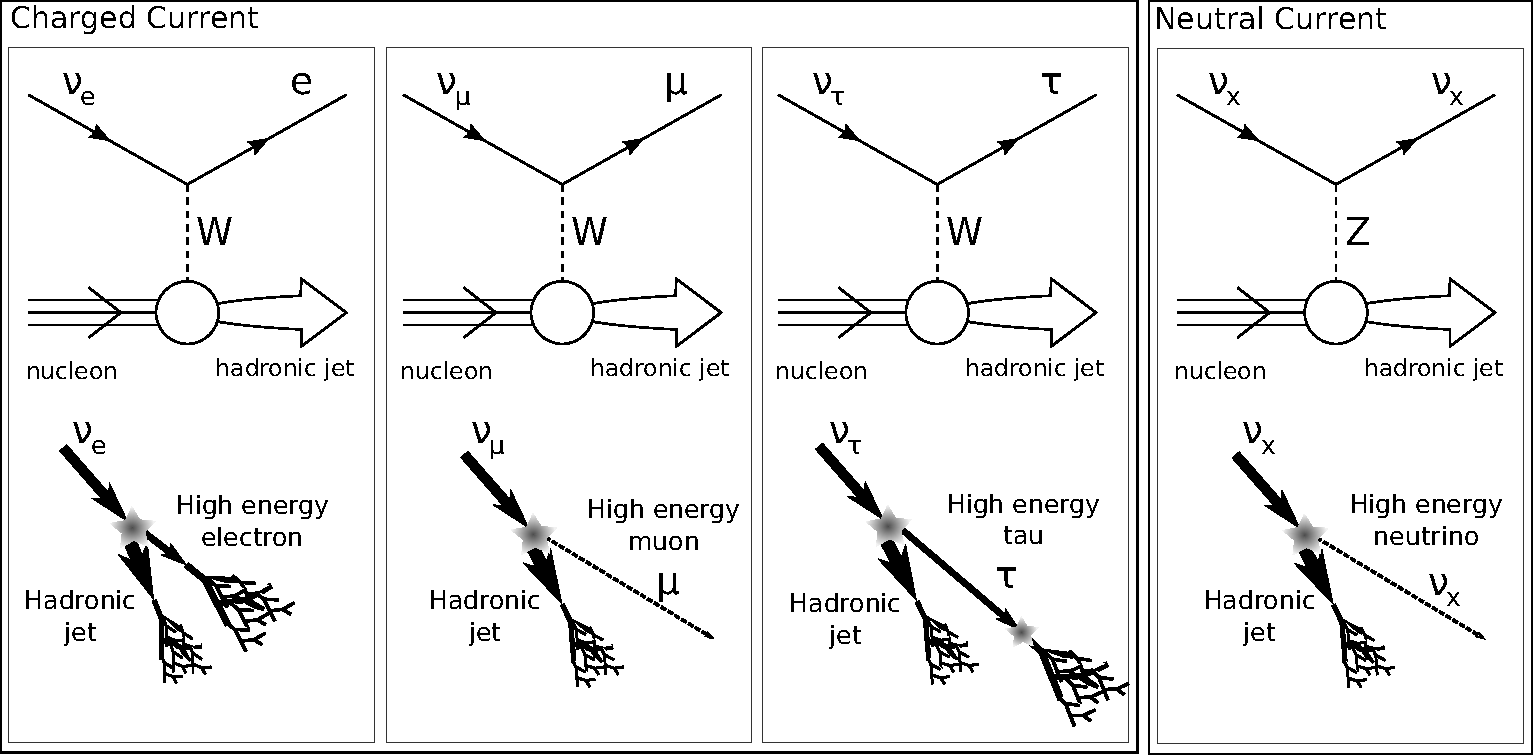
\includegraphics[width=1.0\textwidth]{fig/EASAuger/nu_channels_english.pdf}
\caption{Canales de interacción para neutrinos de acuerdo con el modelo estandar.
En todos los casos se muestra el diagrama de Feynman al orden más bajo.
Para todos los canales, el jet resultante de la fragmentación del núcleo inicia una lluvia hadrónica que posee al rededor del \cant{20}{\%} de la energía del neutrino incidente.
El electrón producido en la interacción via corriente cargada (CC) genera una cascada electromagnética que se suma al jet hadrónico.
Cuando el neutrino primario es un $\nu_{\tau}$ que interactua via CC el $\tau$ generado puede viajar una distancia considerable antes de decaer y generar una cascada, a veces muy cercana al suelo.
Estas se denominan \emph{cascadas double bang}.
Finalmente, en el caso de tener un $\nu_{\mu}$ primario, el $\mu$ resultante en la mayor parte de los casos no genera lluvia alguna.
}
\label{fig:SM_nu_int}
\end{center}
\end{figure}

En el caso de interacción via corriente neutra (NC), luego de perder energía el neutrino escapa sin generar cascada alguna, quedando la cascada con sólo el \cant{20}{\%} de la energía del primario.

Si la lluvia es iniciada por un $\nu_e$ via corriente cargada (CC), el electrón resultante inicia una cascada electromagnética que se superpone con la hadrónica producida por los fragmentos del nucleo.
En este caso, toda la energía del neutrino primario es transferida a la lluvia.

Aunque el mecanismo fundamental mediante el que se inician, Las lluias generadas por $\nu_{\mu}$ via CC son muy similares a las generadas via NC ya que las probabilidades de que el $\mu$ resultante de la interacción decaiga o interactúe antes de llegar al suelo son verdaderamente pequeñas\footnote{La probabilidad de que un $\mu$ de \cant{10^{18}}{eV} decaiga antes de llegar al suelo es de $\sim10^{-6}$ mientras que la probabilidad de que subra DIS o bremsstrahlung es del orden de $10^{-3}$ \cite{cite:tesisJavier}} 

En el caso de un $\nu_{\tau}$ que interactúa via CC el proceso es realmente interesante.
Al igual que el $\mu$, el $\tau$ resultante es una partícula muy penetrante pero con la diferencia de que su vida media es siete ordenes de magnitud menor.
Debido a esto, luego de viajar una distancia considerable (\cant{5}{km} para un $\tau$ de \cant{10^{17}}{eV}) decaerá generando en el \cant{\sim80}{\%} de los casos una cascada detectable, que a su vez será el \cant{\sim25}{\%} de caracter electromagnético y el \cant{\sim75}{\%} restante será hadrónico.
Este tipo de cascadas, muy características, se conocen como ``Double--Bang'' (DB).
%
\begin{figure}[h!]
\begin{center}
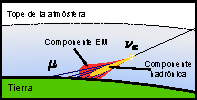
\includegraphics[width=0.7\textwidth]{fig/EASAuger/horizontal_deep_english.pdf}
\caption{Los neutrinos pueden iniciar lluvias inclinadas profundas en la atmósfera.
En este tipo de lluvias tanto la componente electromagnética como la muónica pueden llegar al suelo.
Comparar con la figura \ref{fig:horizontalHad}.
}
\label{fig:horizontalNu}
\end{center}
\end{figure}

El camino libre medio para neutrinos de \cant{10^{18}}{eV} es de \cant{\sim10^8}{gcm^{-2}}\cite{cite:Gandhi}. 
Como este valos es mucho mayor que el ancho de la atmósfera, incluso para $\theta\sim90^\circ$, los neutrinos pueden interactuar básicamente en cualquier punto de la atmósfera con la misma probabilidad.
En particular, pueden iniciar lluvias muy profundo en la atmósfera en las que tanto la componente electromagnética como la muónica puede alcanzar el suelo (ver figura \ref{fig:horizontalNu}).
Por otro lado, esto es practicamente imposible para lluvias iniciadas por hadrones o núcleos, ya que interactúan usualmente en el primer centenar de gramos.
Por esto mismo, la estrategia utilizada para observar neutrinos con detectores de superficie se basa en la detección lluvias inclinadas en las que la componente electromagnética no haya sido absorbida por la atmósfera. Este canal de detección es llamado Down-going (DG).

%
\subsection{Lluvias rasantes iniciadas por neutrinos tau (ES)}
\label{sc:EStauInducedShowers}
%
Otro tipo de lluvias muy interesante son las que pueden ser iniciadas por neutrinos que interactúan en la corteza terrestre.
En este caso, tanto el jet hadrónico producido en la interacción con el núcleo como el electrón producido en el caso de un $\nu_e$ incidente son rápidamente absorbidos por la materia, sin embargo, los leptones $\mu$ y $\tau$ producidos al incidir un $\nu_{\mu}$ o un $\nu_{\tau}$ pueden escapar de la tierra debido a que son muy penetrantes.
Una vez más, debido a su vida media larga, los $\mu$ que escapen de la tierra iniciarán usualmente una luvia muy alto en la atmósfera, por lo que las partículas secundarias rara vez alcanzarán la tierra.
Por otro lado, los leptones $\tau$ tienen baja sección eficaz, lo que les permite escapar de la tierra hacia la atmósfera, pero a su vez poseen un tiempo de vida media que les permite decaer lo suficientemente cerca de la superficie\footnote{La longitud de decaimiento es $\lambda_{d}=c\tau_{\tau}\gamma_{\tau}=49\text{km}\frac{E_{\tau}}{\text{EeV}}$}, iniciando una cascada cuyas partículas secundarias pueden alcanzar el suelo. Este canal de detección es llamado Earth-Skimming (ES) y se esquematiza en la figura \ref{fig:esNu}.

\begin{figure}[ht]
\begin{center}
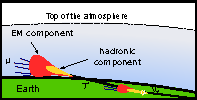
\includegraphics[width=0.7\textwidth]{fig/EASAuger/horizontal_es_english.pdf}
\caption{Un $\nu_{\tau}$ puede interactuar en la tierra via CC dando como resultado un $\tau$ que puede emerger a la atmósfera e iniciar una EAS muy cerca de la superficie de la tierra.
Aunque esta es ascendente, si el $\tau$ emergente posee un ángulo zenital entre $90^\circ$ y $95^\circ$ las partículas que llegan al suelo suelen ser suficientes para ser detectadas.}
\label{fig:esNu}
\end{center}
\end{figure}

Dado que la densidad de la corteza de la tierra es $\sim1000$ veces mayor a la del aire, funciona como un blanco muchísimo mas masivo que la atmósfera para los neutrinos.
Como ejemplo, el camino libre medio para un neutrino de \cant{10^{18}}{eV} en la tierra\footnote{la densidad de la tierra es \cant{\rho_{Earth}\sim2.65}{\frac{g}{cm^3}}} es de \cant{\sim620}{km}.
Por otro lado, bajo la aproximación de tierra esférica, la distancia que debe recorrer un neutrino para atravezarla es $d\sim2R\cos{\theta}$, donde $R$ es el radio de la tierra. 
En consecuencia, como para $91^{\circ}$ se obtiene \cant{d\sim220}{km}, se concluye que \cant{\sim30}{\%} de los neutrinos interactuarán en esas condiciones.
Luego, es necesario considerar la probabilidad de que el $\tau$ escape de la tierra sin perder demasiada energía y a su vez decaiga lo suficientemente cerca del suelo, pero esto se analizará en detalle en la sección \ref{sc:earthInteraction}.

% \section{Detection techniques}
% \label{sec:tecnicasDete}
% 
% \subsection{Surface detector methods}
% %
% As the high energy CR flux is extremly low \footnote{Inferior to one particle per $\rm km^2$ per year.}
% it is necessary to use detectors with an area of several $\rm km^2$ to obtain an amount of data statistically significant.
% 
% The classic way of dealing with the problem is distributing the particle detectors (stations) over a large surface.
% In this way it is possible to sample the secondary particles at different points of the shower front.
% This technique was used by P. Auger and his collaborators when discovering the EAS. 
% In this method, the atmospheric showers are identified when detecting particles in coincidence between two or more stations
% within a time window determined by the distance between them.
% If the shower front is registered by three or more non-aligned stations,
% the direction of the primary particle can be reconstructed from the relative time between the stations (see left panel of Fig.~\ref{fig:tiempoRec}).
% The arrival direction resolution is limited by the time resolution of the stations. When the shower is quasi-horizontal the time difference
% between the stations is given by the distance between stations projected along the direction of the shower, which moves at the speed of light.  
% 
% \begin{figure}
% % 
% % $
% % \begin{array}{cc}
% %  \includegraphics[width=0.47\textwidth]{fig/geome2_english.pdf} & 
% %  \raisebox{0.8\height}{\includegraphics[width=0.47\textwidth]{fig/geome2_es_english.pdf}}
% % \end{array}
% % $
%   \centerline{
%     \mbox{\includegraphics[width=1.0\textwidth]{fig/geome2_inclinedAndHorizontal_english.pdf}}
%     }
%   \caption{ Arrival direction reconstruction scheme using a surface detector array.
% \textit{Left:} Down-going shower.
% \textit{Right:} Quasi-horizontal shower.
% }
%   \label{fig:tiempoRec}
% \end{figure}
% %
% 
% The stations composing the surface array can be of different kinds depending 
% on the charateristics of the shower one wants to measure.
% Nowadays the most common are scintillators and water Cherenkov detectors.
% Scintillators are generally flat surfaces which register particles that go through them. 
% In this way, they allow to measure the particles density by unit of area.
% In most of the atmospheric showers, the amount of photons and electrons is very superior to the other particles.
% For this reason scintillators, if not shielded, are less sensitive to the muonic component. 
% Telescope Array, Yakutsk and AGASA are examples of experiments which chose these kind of detectors~\cite{cite:TA, cite:yakutsk,  cite:agasa}.
% 
% Water Cherenkov detectors were developed by the Haverah Park experiment in the middle of the 60's~\cite{cite:HPark}. 
% These are water tanks that contain inside one or more sensors which register the Cherenkov radiation
% produced by the relativistic particles when they propagate through the water.
% One of the advantages of these detectors is that, being bulky, they are sensitive to particle fluxes very inclined or even horizontal.
% A detailed description of this kind of detector is given in the next chapter. 